\section{Autenticação}
\label{sec:autenticacao}


A autenticação é o processo de verificação da identidade de um usuário ou
sistema.
É uma prova fornecida pelo requerente para afirmar que o usuário em questão
realmente corresponde à identidade fornecida.
O monitor, então, afirma a identidade do usuário.
Os sistemas de autenticação são responsáveis por responder a duas perguntas
fundamentais:
quem é o usuário e o usuário é realmente quem afirma ser?
Assim, a autenticação se apresenta como uma das maneiras mais promissoras de
estabelecer confiança e aprimorar a segurança em aplicações comerciais\cite{
    idrus2013}.

A identificação, a autenticação e a autorização são frequentemente integradas em
sistemas de segurança do mundo real.
Por exemplo, um agente de segurança que monitora o acesso a uma instalação
reconhece as pessoas que trabalham lá (identificação e autenticação) e permite
que elas entrem (autorização) somente porque o agente reconhece os rostos.
Na era digital, os três processos devem ser únicos para serem viáveis
\cite[p.97]{renaud2004}.

\begin{figure}[h!]
    \caption[Áreas de preocupação]
    {Áreas de preocupação durante um processo de autenticação}
    \begin{adjustbox}{width=0.6\columnwidth, center}
        \begin{tikzpicture}[
            db/.style={cylinder,
            draw,
            cylinder uses custom fill,
            cylinder body fill=yellow!20,
            cylinder end fill=yellow!40,
            aspect=0.25,
            text width=2.5cm,
            align=center,
            shape border rotate=90,
            },
            parallelogram/.style={
                trapezium,
                trapezium stretches=false,
                trapezium left angle=60,
                trapezium right angle=120,
            }
        ]
            \node[draw,align=center, text width=2.5cm](auth){Mecanismos de
            Autenticação};
            \node[draw,rounded corners=1mm](server)[right=1cm of auth]{Servidor};
            \node[draw,db](db)[right=1cm of server]{Armazenamento de arquivos};
            \node[draw,parallelogram](input)[below=0.5cm of auth]{Mecanismo de
            entrada};
            
            \draw[thick, ->] (input) edge (auth);
            \draw[thick, ->] (auth)  edge (server);
            \draw[dashed, -] (server) edge (db);
            
            \draw[thick,-](-3,-2) -- (-3,-4.5);
            \draw[thick,-](8,-2) -- (8,-4.5);
            
            \draw(-1.5,-2.5) node[align=center,text width=1.5cm](human){Fatores
            Humanos};
            \draw[thick, ->](human) -- (-3, -2.5);
            \draw[thick, ->](human) -- (0, -2.5);
            
            \draw[thick, -](0,-2) -- (0, -3);
            
            \draw(4, -2.5) node(tech){Tecnologia};
            \draw[thick, ->] (tech) -- (0, -2.5);
            \draw[thick, ->] (tech) -- (8, -2.5);
            
            \draw(0.25, -3.5) node{Acessibilidade};
            \draw[thick, -] (-1.5, -3.2) -- (-1.5, -3.9);
            \draw[thick, -] (2, -3.2) -- (2, -3.9);
            \draw[thick, <->] (-1.5, -3.8) -- (2, -3.8);
            
            \draw(2.5, -4.25) node(security){Segurança e Vulnerabilidade};
            \draw[thick, ->](security) -- (-3,-4.25);
            \draw[thick, ->](security) -- (8,-4.25);
        
        \end{tikzpicture}
    \end{adjustbox}
    \floatfoot{Adaptado de \cite{renaud2004}}
\end{figure}
Normalmente, a autenticação ocorre quando um usuário chega a uma interface de
login e insere nome de usuário e senha, ou outro token seguro.
Depois disso, é feita uma comparação entre essas credenciais e as credenciais
mantidas em um banco de dados de serviços de diretório que serve como fonte
autorizada para a autenticação da identidade do usuário.
Basicamente, o usuário recebe acesso se as credenciais apresentadas
corresponderem às credenciais mantidas no banco de dados de serviços de
diretório, caso contrário, o acesso é negado\cite[p.112]{alnaji2020}.

Existem várias metodologias de autenticação distintas,
tais como autenticação estática por meio de um segredo compartilhado;
\textit{token} de senha única; autenticação baseada em desafio-resposta
criptográfica;
identificação por radiofrequência; e biometria.
O mecanismo de autenticação mais popular é a conhecida combinação de~\acrfull{id} e senha.
Embora seja obviamente inseguro, é comumente utilizado.
Isso se deve à simplicidade de uso da solução e ao reconhecimento imediato pelos
usuários, facilitando a implantação e aceitação\cite{idrus2013}.
\subsection{Autenticação estática via segredo compartilhado}
\label{subsec:autenticacao-estatica-segredo-compartilhado}

A autenticação estática é amplamente utilizada na forma de autenticação baseada
em formulário de~\acrshort{id} e senha, sendo considerada a aplicação mais
conhecida.
Nesse método, o solicitante confirma sua identidade ao monitor, demonstrando
conhecimento de um segredo compartilhado, geralmente revelando-o para eles\cite{idrus2013}.

A autenticação estática geralmente funciona da
seguinte forma: o requerente verifica para o requerido que está ciente de um
segredo
compartilhado, geralmente divulgando-o para tal.
O requerido então determina se é o valor correto comparando-o com um mantido em
um banco de dados de verificação\cite{idrus2013}.

\begin{figure}[h!]
    \caption[Diagrama representação autenticação de \acrshort{id} e senha]
    {Diagrama de transição de estados representando autenticação com
    \acrshort{id} e senha}
    \begin{tikzpicture}
    [
        action/.style={draw, very thick, rounded corners, text width=2.5cm,
        align=center},
        initial/.style={draw, circle, fill, minimum size=10mm},
        final/.style={draw, double, thick, circle, fill, minimum size=10mm},
        decision/.style={draw, diamond, black, fill, minimum size=10mm},
    ]
        \node[initial](init);
        \node[action](provision)[right=0.5cm of init]{O usuário fornece nome de
        usuário e senha.};
        \node[decision, label={
            [text width=2.5cm, xshift=0.5cm]Nome de usuário e senha corretos?}]
        (validation)[right=0.5cm of provision];
        \node[action, text width=3cm](error)[below=1cm of validation]
        {Nome de usuário e/ou senha inválidos. Solicite ao usuário novamente.}
        \node[action](success)[right=1.5cm of validation]
        {Autenticação do usuário bem-sucedida. Garantir acesso.};
        \node[final](end)[right=0.5cm of success];
        
        \draw[thick, ->](init) edge (provision);
        \draw[thick, ->](provision) edge (validation);
        \draw[thick, ->](validation) --node[center, fill=white]{sim} (success);
        \draw[thick, ->](validation) --node[center, fill=white]{não} (error);
        \draw[thick, ->](error) -| (provision);
        \draw[thick, ->](success) edge (end);
    \end{tikzpicture}
    \floatfoot{Adaptado de \cite{horsh2018}}
    \label{fig:diagrama-autenticacao-id-senha}
\end{figure}

A autenticação de usuários baseada em senhas em sistemas computacionais tem
sido a base da segurança de computadores por muitos anos.
Para manter um segredo compartilhado entre um usuário e um sistema de
computador,
a ideia de um \acrshort{id} e senha é prática e econômica\cite{conklin2004}.

Do ponto de vista dos aplicativos, era lógico adotar a autenticação de usuário
baseada em senha quando havia menos aplicativos em comparação com o número de
usuários.
No entanto, essa suposição de que cada usuário possui um número limitado de
programas
não é mais válida devido ao crescimento da Internet e à tendência de computa
ção ubíqua.
Em muitos sistemas, os usuários têm várias contas e precisam memorizar diversos
IDs e senhas\cite{conklin2004}.
\subsection{Autenticação via \texit{token} de senha única}
\label{subsec:autenticacao-token-senha-unica}

Os \textit{tokens} de senha única ou~\acrfull{otp} são senhas dinâmicas criadas
por um sistema gerador, no qual são capazes serem utilizadas apenas uma vez e
por um período limitado, restringindo a janela de oportunidade para
um atacante agir\cite{christiana2019}.

Segundo~\textcite{huiyi2013}, a geração de~\acrshort{otp} pode ser realizada
por meio de métodos de hash como~\acrfull{sha1} ou~\acrfull{md5}, assim como por
meio de inteiros aleatórios ou contadores que aumentam a cada uso, a fim de
sincronizar o tempo entre o usuário e o servidor.

Os sistemas~\acrshort{otp} podem ser entendidos como uma ponte entre um
mecanismo de autenticação mais seguro e a autenticação estática por senha.
Isso facilita a migração de aplicativos legados, como unidades centrais de
processamento (\textit{mainframes}) e sites, que foram originalmente projetados
para funcionar apenas com senhas\cite{idrus2013}.

Porém, os sistemas~\acrshort{otp} contém algumas vulnerabilidades também.
Segundo~\textcite{hoyul2015} existem certas vulnerabilidades no~\acrshort{otp
} que o tornam
suscetível a ataques~\acrfull{mitm} e ataques~\acrfull{mitpcp1}.
Durante a fase de inicialização do algoritmo~\acrshort{otp}, um servidor e os
clientes trocam certos dados confidenciais.
Um invasor pode efetivamente se autenticar se ele usar um ataque~\acrshort{mitm}
para obter algumas informações confidenciais.
Um invasor também pode obter acesso à memória do dispositivo e
produzir valores~\acrshort{otp} se ele implantar código malicioso nos
dispositivos dos usuários\cite{hoyul2015}.
\subsection{Autenticação Baseada em Desafio-Resposta}
\label{subsec:autenticacao-desafio-resposta}

O~\acrfull{cram}, ou mecanismo de autenticação desafio-resposta, é um
procedimento
cujo objetivo é verificar a autenticidade de uma entidade que solicita acesso,
exigindo que ela demonstre estar ciente de um segredo, sem revelá-lo ao
verificador.
O procedimento consiste no verificador oferecendo um desafio ao solicitante a
partir de um conjunto de desafios preparados.
O solicitante recebe um desafio que varia ao longo do tempo do verificador e,
em resposta, utiliza uma função dependente do segredo para gerar uma resposta.
Caso o solicitante responda corretamente ao desafio oferecido, ele é autenticado
e recebe acesso a um computador, rede ou outro recurso\cite{gilad2013}.

\begin{figure}[h!]
    \centering
    \caption[Diagrama representação autenticação via desafio-resposta]
    {Diagrama de transição de estados representando autenticação com
    desafio-resposta}
    \begin{tikzpicture}
    [
        action/.style={draw, very thick, rounded corners, text width=1.5cm,
        align=center},
        initial/.style={draw, circle, fill, minimum size=10mm},
        final/.style={draw, double, thick, circle, fill, minimum size=10mm},
        decision/.style={draw, diamond, black, fill, minimum size=10mm},
    ]
        \node[initial](begin);
        \node[action](request)[right=0.5cm of begin]
        {Solicitação de autenticação.};
        \node[action](challenge)[right=0.5cm of request]
        {Desafio enviado ao usuário.};
        \node[decision, label={
            [text width=2.5cm, align=center]
            O usuário tenta fazer o desafio, a resposta está correta?}]
        (attempt)[right=0.75cm of challenge];
        \node[action](success)[right=1.25cm of attempt]{Acesso garantido.};
        \node[final](end)[right=0.5cm of success];
        
        \draw[thick, ->](begin) edge (request);
        \draw[thick, ->](request) edge (challenge);
        \draw[thick, ->](challenge) edge (attempt);
        \draw[thick, ->](attempt) -- node[center, fill=white]{sim}(success);
        \draw[thick, ->](attempt.south) |- (5,-2)
        node[center, above, xshift=0.25cm,fill=white]{não} -| (challenge.south);
        \draw[thick, ->](success) edge (end);
    \end{tikzpicture}
    \floatfoot{Adaptado de \cite{gilad2013}}
    \label{fig:diagrama-autenticacao-desafio-resposta}
\end{figure}

Segundo~\textcite{idrus2013} caso seja executada de forma adequada, a
autenticação
via desafio-resposta criptográfica se mostra uma abordagem de autenticação
extremamente
eficiente e confiável.
No entanto, a manutenção pode exigir um grande investimento de tempo, energia e
recursos financeiros.
\subsection{Autenticação via identificação por radiofrequência}
\label{subsec:autenticacao-identificacao-radiofrequencia}

Os sistemas de identificação por radiofrequência ou~\acrfull{rfid} são uma
tecnologia
utilizada para recuperar informações automaticamente sobre produtos, pessoas ou
animais - ou seja, qualquer objeto em geral.
O objeto possui um pequeno circuito conhecido como \textit{tag}~\acrshort{
    rfid}, e os
dados registrados no meio podem ser recuperados automaticamente por um
dispositivo leitor.
Essa característica pode ser empregada em diversas aplicações industriais,
como rastreamento de itens ou sistemas de controle de acesso.
Além disso, os sistemas~\acrshort{rfid} não requerem contato, e nem precisam
estar
no campo de visão, utilizando a radiofrequência para transportar dados e energia
de forma eficiente\cite{feldhofer2004}.

\begin{figure}[h!]
    \caption[Estrutura de um sistema~\acrshort{rfid}]
    {Estrutura de um sistema~\acrshort{rfid}}
    \begin{tikzpicture}
    [
        action/.style={
            draw, thick, rectangle, rounded corners,
            text width=1.5cm, align=center,
        },
        action2/.style={
            draw, thick, double arrow,
            text width=1cm, align=center
        },
        snake/.style={
            -,
            decorate,
            decoration={
                snake,
                amplitude=1mm,
            }
        }
    ]
        \node[label={[below, yshift=-1.2cm,align=center]\textit{host}}](host){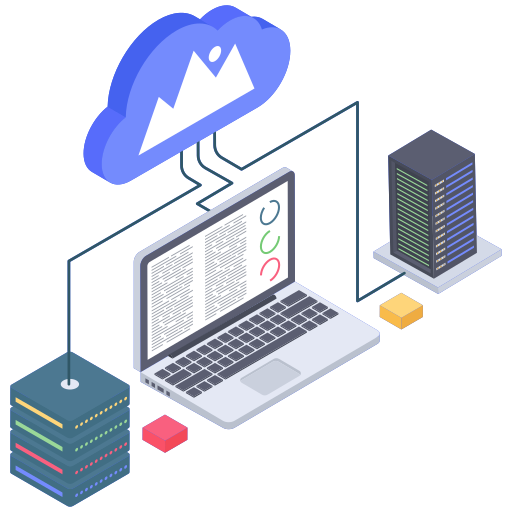
\includegraphics[width=0.1\textwidth]{graphics/host}};
        \node[action](reader)[right=0.8cm of host]{Leitor};
        \node[label={[above, align=center] Antena}](antenna)[right=0.1cm of
        reader]{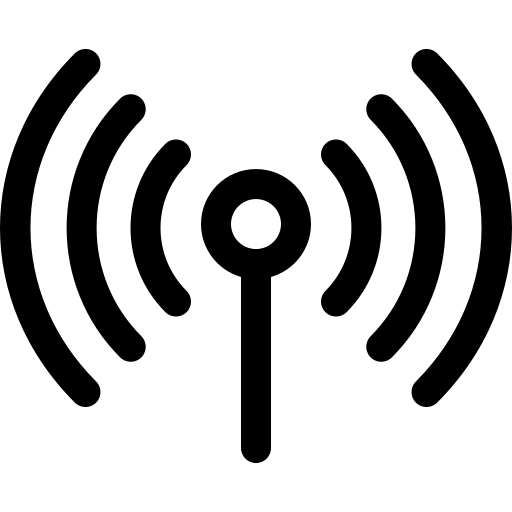
\includegraphics[width=0.05\textwidth]{graphics/antenna}};
        \node[action2](object)[right=0.3cm of antenna]{Dados \\ Energia \\
        Relógio};
        \node[action](tag)[right=1cm of object]{\textit{tag}}
        \node[label={[above, align=center] Antena}](antenna2)[left=0.1cm of
        tag]{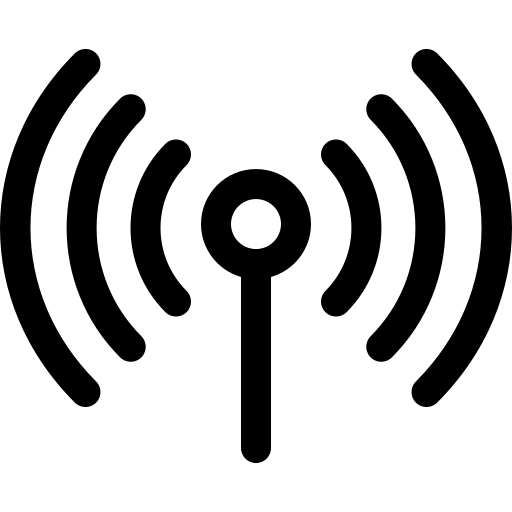
\includegraphics[width=0.05\textwidth]{graphics/antenna}};
        
        \draw (host) edge[snake] (reader);
    \end{tikzpicture}
    \label{fig:estrutura-sistema-rfid}
    \floatfoot{Adaptado de \cite{feldhofer2004}}
\end{figure}

Nos anos 50, os primeiros \textit{tags}~\acrshort{rfid} foram utilizados para
fins militares, embora fossem apenas para identificação.
Na época, sua função era limitada a transmitir sem fio um número serial
por ondas de rádio.
Nos últimos anos, os \textit{tags}~\acrshort{rfid} são um enorme sucesso na
indústria e seu uso se tornou generalizado.
As \textit{tags}~\acrshort{rfid} têm uma ampla gama de aplicações, incluindo
identificação de itens para dados de inventário, gerenciamento da cadeia de
suprimentos, telefones com capacidades~\acrshort{rfid} e autenticação de cartões
de plástico.
Acredita-se que dependemos da Internet para tudo e os \textit{tags}~\acrshort{rfid}
ajudarão nessa transição, dando capacidades de comunicação a produtos
cotidianos\cite{idrus2013}.

A segurança e o custo são duas desvantagens do~\acrshort{rfid}RFID.
Embora o custo do~\acrshort{rfid} seja relativamente baixo em comparação com
outros sistemas de identificação, ainda é um pouco mais caro do que os sistemas
de código de barras convencionais.
As \textit{tags}~\acrshort{rfid} são vulneráveis a múltiplos ataques, representando
um risco de privacidade.
Portanto, muitos acadêmicos enfrentam o desafio de aumentar a segurança do~\acrshort{rfid},
enquanto mantêm o baixo custo das \textit{tags}~\acrshort{rfid}, determinando o
melhor método de autenticação\cite{jadhao2018}.
\subsection{Autenticação Biométrica}
\label{subsec:autenticacao-biometrica}

A biometria é uma técnica utilizada na ciência da computação para controlar o
acesso e gerenciar a identidade de usuários.
O termo biometria tem origem no grego antigo sendo composto pelos termos \textit{bios},
que significa vida, e \textit{metron}, que se refere à medição.
A ciência da biometria estuda como identificar indivíduos por meio de
características físicas ou comportamentais\cite{idrus2013}.

Portanto, a autenticação biométrica ou biometria é o processo pelo qual
computadores
são utilizados para identificar indivíduos, apesar das diferenças existentes
de cada um.
Cada técnica biométrica é incapaz de determinar a identidade "verdadeira" de um
indivíduo.
Em vez disso, a identificação de uma pessoa e quaisquer características pessoais
fornecidas no momento da inscrição no sistema são as únicas informações que a
tecnologia biométrica pode associar a elas, além de um padrão biométrico\cite{wayman2005}.

A natureza humana faz com que as pessoas confiem naturalmente nas características
físicas do corpo humano que são visíveis, como as feições do rosto, a voz, o
caminhar,
a assinatura, entre outros.
Como esses traços são particulares de cada indivíduo, esses métodos são
excelentes para identificar outras pessoas\cite{alsaadi2015}.

\begin{figure}[h!]
    \caption[Classificação geral dos sistemas biométricos]{Classificação
    geral dos sistemas biométricos}
    \begin{adjustbox}{width=0.8\columnwidth, center}
        \begin{tikzpicture}[
            action/.style={draw, very thick, rounded corners,
            text width=2.5cm,
            align=center}
        ]
            \node[action](main){Autenticação baseada em biometria};
            \node[action](physiological)[below left=1cm and 0.1cm of main]
            {Fisiológico};
            \node[action](behavioral)[below right=1cm and 0.1cm of main]
            {Comportamental};
            \node(p-childs)[below=1cm of physiological]{
                \begin{tblr}{|c|}
                    \hline
                    Reconhecimento de faces   \\ \hline
                    Geometria da mão          \\ \hline
                    Impressão digital         \\ \hline
                    Íris                      \\ \hline
                    Retina                    \\ \hline
                    Reconhecimento de orelhas \\ \hline
                \end{tblr}
            }
            \node(b-childs)[below=1cm of behavioral]{
                \begin{tblr}{|c|}
                    \hline
                    Voz            \\ \hline
                    Assinatura     \\ \hline
                    Marcha         \\ \hline
                    Toque de tecla \\ \hline
                    Dinâmica       \\ \hline
                    Lábios         \\ \hline
                    Movimentos     \\ \hline
                \end{tblr}
            }
            
            \draw[thick] (main.south) -| (0, -1) edge[->] (physiological.north);
            \draw[thick] (main.south) -| (0, -1) edge[->] (behavioral.north);
            \draw[thick, ->](physiological) edge (p-childs);
            \draw[thick, ->](behavioral) edge (b-childs);
        \end{tikzpicture}
    \end{adjustbox}
    \floatfoot{Adaptado de \cite{alsaadi2015}}
\end{figure}
A principal vantagem dessas técnicas de autenticação é a estreita conexão que
existe entre o usuário e o autenticador, que é o dado biométrico.
Além disso, ao contrário da maioria das outras técnicas de autenticação,
é difícil replicar as características biométricas de um indivíduo.
No entanto, a autenticação biométrica tem uma desvantagem, que é a
imprevisibilidade
do resultado de verificação.
Por exemplo, na autenticação por impressão digital, um erro pode ocorrer devido
ao alinhamento inadequado do dedo\cite{idrus2013}.